\chapter{Polishing your plots for publication}\label{cha:polishing}

In this chapter you will learn how to prepare polished plots for
publication. Most of this chapter focusses on the theming capability of
\texttt{ggplot} which allows you to control many non-data aspects of
plot appearance, but you will also learn how to adjust geom, stat and
scale defaults, and the best way to save plots for inclusion into other
software packages. Together with the next chapter, manipulating plot
rendering with \textbf{grid}, you will learn how to control every visual
aspect of the plot to get exactly the appearance that you want.
\index{Publication!polishing plots for}

The visual appearance of the plot is determined by both data and
non-data related components. \hyperref[sec:themes]{Themes} introduces
the theme system which controls all aspects of non-data display. By now
you should be familiar with the many ways that you can alter the
data-related components of the plot---layers and scales---to visualise
your data and change the appearance of the plot. In
\hyperref[sec:theme-scale-geom]{customising scales and geoms} you will
learn how you can change the defaults for these, so that you do not need
to repeat the same parameters again and again.

\hyperref[sec:saving]{Saving your output} discusses the chapter with a
discussion about how to get your graphics out of R and into LaTeX, Word
or other presentation or word-processing software.
\hyperref[sec:grid-layout]{Multiple plots on the same page} concludes
with a discussion of how to lay out multiple plots on a single page.

\hyperdef{}{sec:themes}{\section{Themes}\label{sec:themes}}

The appearance of non-data elements of the plot is controlled by the
theme system. The theme system does not affect how the data is rendered
by geoms, or how it is transformed by scales. Themes don't change the
perceptual properties of the plot, but they do help you make the plot
aesthetically pleasing or match existing style guides. Themes give you
control over things like the fonts in all parts of the plot: the title,
axis labels, axis tick labels, strips, legend labels and legend key
labels; and the colour of ticks, grid lines and backgrounds (panel,
plot, strip and legend). \index{Themes} \index{Publication!themes}

This separation of control into data and non-data parts is quite
different than base and lattice graphics. In base and lattice graphics,
most functions take a large number of arguments that specify both data
and non-data appearance, which makes the functions complicated and hard
to learn. ggplot takes a different approach: when creating the plot you
determine how the data is displayed, then \emph{after} it has been
created you can edit every detail of the rendering, using the theming
system. Some of the effects of changing the theme of a plot are shown in
Figure \ref{fig:themes}. The two plots show the two themes included by
default in ggplot.

\begin{figure}

{\centering \includegraphics[width=0.49\linewidth]{figures/polishingthemes-1} \includegraphics[width=0.49\linewidth]{figures/polishingthemes-2} 

}

\caption{The effect of changing themes.  (Left) The default grey theme with grey background and white gridlines.  (Right) the alternative black and white theme with white background and grey gridlines.  Notice how the bars, data elements, are identical in both plots.\label{fig:themes}}
\end{figure}

Like many other areas of \texttt{ggplot}, themes can be controlled on
multiple levels from coarse to fine. You can:

\begin{itemize}
\itemsep1pt\parskip0pt\parsep0pt
\item
  Use a built-in theme. This affects every element of the plot in a
  visually consistent manner. The default theme uses a grey panel
  background with white gridlines; however, there are built-in
  alternatives such as \texttt{theme\_bw()} which uses a white
  background with grey gridlines (\hyperref[sec:built-in]{link to
  section}).
\item
  Modify a single element of a built-in theme. Each theme is made up of
  multiple elements. The theme system comes with a number of built-in
  element rendering functions with a limited set of parameters. By
  adjusting these parameters you can control things like text size and
  colour, background and grid line colours and text orientation. By
  combining multiple elements you can create your own theme
  (\hyperref[sec:theme-elements]{link to section}).
\end{itemize}

Generally each of these theme settings can be applied globally, to all
plots, or locally to a single plot. How to do this is described in each
section.

\hyperdef{}{sec:built-in}{\subsection{Built-in
themes}\label{sec:built-in}}

There are two built-in themes. \index{Themes!built-in} The default,
\texttt{theme\_gray()}, uses a very light grey background with white
gridlines. This follows from the advice of (Tufte 2006; Tufte 1990;
Tufte 2001; Tufte 1997) and (Brewer 1994; Carr 2002; Carr 1994; Carr and
Sun 1999). We can still see the gridlines to aid in the judgement of
position (Cleveland 1993), but they have little visual impact and we can
easily `tune' them out. The grey background gives the plot a similar
colour (in a typographical sense) to the remainder of the text, ensuring
that the graphics fit in with the flow of a text without jumping out
with a bright white background. Finally, the grey background creates a
continuous field of colour which ensures that the plot is perceived as a
single visual entity. \indexf{theme_grey}

The other built-in theme, \texttt{theme\_bw()}, has a more traditional
white background with dark grey gridlines. Figure \ref{fig:themes} shows
some of the difference between these themes. \index{White background}
\index{Themes!white background} \indexf{theme_bw}

Both themes have a single parameter, \texttt{base\_size}, which controls
the base font size. The base font size is the size that the axis titles
use: the plot title is 20\% bigger, and the tick and strip labels are
20\% smaller. If you want to control these sizes separately, you'll need
to modify the individual elements as described in the following section.

You can apply themes in two ways:

\begin{itemize}
\itemsep1pt\parskip0pt\parsep0pt
\item
  Globally, affecting all plots when they are drawn:
  \texttt{theme\_set(theme\_grey())} or
  \texttt{theme\_set(theme\_bw())}. \texttt{theme\_set()} returns the
  previous theme so that you can restore it later if you want.
  \indexf{theme_set}
\item
  Locally, for an individual plot: \texttt{qplot(...) + theme\_grey()}.
  A locally applied theme will override the global default.
\end{itemize}

The following example shows a few of these combinations:

\begin{Shaded}
\begin{Highlighting}[]
\NormalTok{>}\StringTok{ }\NormalTok{hgram <-}\StringTok{ }\KeywordTok{qplot}\NormalTok{(rating, }\DataTypeTok{data =} \NormalTok{movies, }\DataTypeTok{binwidth =} \DecValTok{1}\NormalTok{)}
\NormalTok{>}\StringTok{ }
\ErrorTok{>}\StringTok{ }\CommentTok{# Themes affect the plot when they are drawn, }
\ErrorTok{>}\StringTok{ }\CommentTok{# not when they are created}
\ErrorTok{>}\StringTok{ }\NormalTok{hgram}
\end{Highlighting}
\end{Shaded}

\begin{flushleft}\includegraphics[width=0.49\linewidth]{figures/polishinghgram-1} \end{flushleft}

\begin{Shaded}
\begin{Highlighting}[]
\NormalTok{>}\StringTok{ }\NormalTok{previous_theme <-}\StringTok{ }\KeywordTok{theme_set}\NormalTok{(}\KeywordTok{theme_bw}\NormalTok{())}
\NormalTok{>}\StringTok{ }\NormalTok{hgram}
\end{Highlighting}
\end{Shaded}

\begin{flushleft}\includegraphics[width=0.49\linewidth]{figures/polishinghgram-2} \end{flushleft}

\begin{Shaded}
\begin{Highlighting}[]
\NormalTok{>}\StringTok{ }
\ErrorTok{>}\StringTok{ }\CommentTok{# You can override the theme for a single plot by adding }
\ErrorTok{>}\StringTok{ }\CommentTok{# the theme to the plot. Here we apply the original theme}
\ErrorTok{>}\StringTok{ }\NormalTok{hgram +}\StringTok{ }\NormalTok{previous_theme}
\end{Highlighting}
\end{Shaded}

\begin{flushleft}\includegraphics[width=0.49\linewidth]{figures/polishinghgram-3} \end{flushleft}

\begin{Shaded}
\begin{Highlighting}[]
\NormalTok{>}\StringTok{ }
\ErrorTok{>}\StringTok{ }\CommentTok{# Permanently restore the original theme}
\ErrorTok{>}\StringTok{ }\KeywordTok{theme_set}\NormalTok{(previous_theme)}
\end{Highlighting}
\end{Shaded}

\hyperdef{}{sec:theme-elements}{\subsection{Theme elements and element
functions}\label{sec:theme-elements}}

A theme is made up of multiple \emph{elements} which control the
appearance of a single item on the plot, as listed in
Table\textasciitilde{}\ref{tbl:elements}. There are three elements that
have individual \texttt{x} and \texttt{y} settings: \texttt{axis.text},
\texttt{axis.title} and \texttt{strip.text}. Having a different setting
for the horizontal and vertical elements allows you to control how text
should appear in different orientations. The appearance of each element
is controlled by an \emph{element function}. \index{Themes!elements}
There are four basic types of built-in element functions: text, lines
and segments, rectangles and blank. Each element function has a set of
parameters that control the appearance as described below:

\begin{itemize}
\itemsep1pt\parskip0pt\parsep0pt
\item
  \texttt{element\_text()} draws labels and headings. You can control
  the font \texttt{family}, \texttt{face}, \texttt{colour},
  \texttt{size}, \texttt{hjust}, \texttt{vjust}, \texttt{angle} and
  \texttt{lineheight}. \index{Themes!labels} \indexf{element_text}
\end{itemize}

The following code shows the effect of changing these parameters on the
plot title. The results are shown in Figure \ref{fig:theme-text}.
Changing the angle is probably more useful for tick labels. When
changing the angle you will probably also need to change \texttt{hjust}
to 0 or 1.

\begin{Shaded}
\begin{Highlighting}[]
\NormalTok{hgramt <-}\StringTok{ }\NormalTok{hgram +}\StringTok{ }\KeywordTok{labs}\NormalTok{(}\DataTypeTok{title =} \StringTok{"This is a histogram"}\NormalTok{)}
\NormalTok{hgramt}
\NormalTok{hgramt +}\StringTok{ }\KeywordTok{theme}\NormalTok{(}\DataTypeTok{plot.title =} \KeywordTok{element_text}\NormalTok{(}\DataTypeTok{size =} \DecValTok{20}\NormalTok{))}
\NormalTok{hgramt +}\StringTok{ }\KeywordTok{theme}\NormalTok{(}\DataTypeTok{plot.title =} 
              \KeywordTok{element_text}\NormalTok{(}\DataTypeTok{size =} \DecValTok{20}\NormalTok{, }\DataTypeTok{colour =} \StringTok{"red"}\NormalTok{))}
\NormalTok{hgramt +}\StringTok{ }\KeywordTok{theme}\NormalTok{(}\DataTypeTok{plot.title =} 
              \KeywordTok{element_text}\NormalTok{(}\DataTypeTok{size =} \DecValTok{20}\NormalTok{, }\DataTypeTok{hjust =} \DecValTok{0}\NormalTok{))}
\NormalTok{hgramt +}\StringTok{ }\KeywordTok{theme}\NormalTok{(}\DataTypeTok{plot.title =} 
              \KeywordTok{element_text}\NormalTok{(}\DataTypeTok{size =} \DecValTok{20}\NormalTok{, }\DataTypeTok{face =} \StringTok{"bold"}\NormalTok{))}
\NormalTok{hgramt +}\StringTok{ }\KeywordTok{theme}\NormalTok{(}\DataTypeTok{plot.title =} 
              \KeywordTok{element_text}\NormalTok{(}\DataTypeTok{size =} \DecValTok{20}\NormalTok{, }\DataTypeTok{angle =} \DecValTok{180}\NormalTok{))}
\end{Highlighting}
\end{Shaded}

\begin{figure}

{\centering \includegraphics[width=0.32\linewidth]{figures/polishingtheme-text-1} \includegraphics[width=0.32\linewidth]{figures/polishingtheme-text-2} \includegraphics[width=0.32\linewidth]{figures/polishingtheme-text-3} \includegraphics[width=0.32\linewidth]{figures/polishingtheme-text-4} \includegraphics[width=0.32\linewidth]{figures/polishingtheme-text-5} \includegraphics[width=0.32\linewidth]{figures/polishingtheme-text-6} 

}

\caption{Changing the appearance of the plot title.\label{fig:theme-text}}
\end{figure}

\begin{itemize}
\itemsep1pt\parskip0pt\parsep0pt
\item
  \texttt{element\_line()} draws lines with the same options but in a
  slightly different way. Make sure you match the appropriate type or
  you will get strange grid errors. For these element functions you can
  control the \texttt{colour}, \texttt{size} and \texttt{linetype}.
  These options are illustrated with the code and the results are shown
  in Figure \ref{fig:theme-line}. \indexf{element_line}
\end{itemize}

\begin{Shaded}
\begin{Highlighting}[]
\NormalTok{hgram +}\StringTok{ }\KeywordTok{theme}\NormalTok{(}\DataTypeTok{panel.grid.major =} \KeywordTok{element_line}\NormalTok{(}\DataTypeTok{colour =} \StringTok{"red"}\NormalTok{))}
\NormalTok{hgram +}\StringTok{ }\KeywordTok{theme}\NormalTok{(}\DataTypeTok{panel.grid.major =} \KeywordTok{element_line}\NormalTok{(}\DataTypeTok{size =} \DecValTok{2}\NormalTok{))}
\NormalTok{hgram +}\StringTok{ }\KeywordTok{theme}\NormalTok{(}\DataTypeTok{panel.grid.major =} \KeywordTok{element_line}\NormalTok{(}\DataTypeTok{linetype =} \StringTok{"dotted"}\NormalTok{))}
\NormalTok{hgram +}\StringTok{ }\KeywordTok{theme}\NormalTok{(}\DataTypeTok{axis.line =} \KeywordTok{element_line}\NormalTok{())}
\NormalTok{hgram +}\StringTok{ }\KeywordTok{theme}\NormalTok{(}\DataTypeTok{axis.line =} \KeywordTok{element_line}\NormalTok{(}\DataTypeTok{colour =} \StringTok{"red"}\NormalTok{))}
\NormalTok{hgram +}\StringTok{ }\KeywordTok{theme}\NormalTok{(}\DataTypeTok{axis.line =} \KeywordTok{element_line}\NormalTok{(}\DataTypeTok{size =} \FloatTok{0.5}\NormalTok{, }\DataTypeTok{linetype =} \StringTok{"dashed"}\NormalTok{))}
\end{Highlighting}
\end{Shaded}

\begin{figure}

{\centering \includegraphics[width=0.32\linewidth]{figures/polishingtheme-line-1} \includegraphics[width=0.32\linewidth]{figures/polishingtheme-line-2} \includegraphics[width=0.32\linewidth]{figures/polishingtheme-line-3} \includegraphics[width=0.32\linewidth]{figures/polishingtheme-line-4} \includegraphics[width=0.32\linewidth]{figures/polishingtheme-line-5} \includegraphics[width=0.32\linewidth]{figures/polishingtheme-line-6} 

}

\caption{Changing the appearance of lines and segments in the plot.\label{fig:theme-line}}
\end{figure}

\begin{itemize}
\itemsep1pt\parskip0pt\parsep0pt
\item
  \texttt{element\_rect()} draws rectangles, mostly used for
  backgrounds, you can control the \texttt{fill} colour and border
  \texttt{colour}, \texttt{size} and \texttt{linetype}. Examples shown
  in Figure \ref{fig:theme-background} are created with the code below:
  \index{Background} \index{Themes!background} \indexf{theme_rect}
\end{itemize}

\begin{Shaded}
\begin{Highlighting}[]
\NormalTok{hgram +}\StringTok{ }\KeywordTok{theme}\NormalTok{(}\DataTypeTok{plot.background =} \KeywordTok{element_rect}\NormalTok{(}\DataTypeTok{fill =} \StringTok{"grey80"}\NormalTok{, }\DataTypeTok{colour =} \OtherTok{NA}\NormalTok{))}
\NormalTok{hgram +}\StringTok{ }\KeywordTok{theme}\NormalTok{(}\DataTypeTok{plot.background =} \KeywordTok{element_rect}\NormalTok{(}\DataTypeTok{size =} \DecValTok{2}\NormalTok{))}
\NormalTok{hgram +}\StringTok{ }\KeywordTok{theme}\NormalTok{(}\DataTypeTok{plot.background =} \KeywordTok{element_rect}\NormalTok{(}\DataTypeTok{colour =} \StringTok{"red"}\NormalTok{))}
\NormalTok{hgram +}\StringTok{ }\KeywordTok{theme}\NormalTok{(}\DataTypeTok{panel.background =} \KeywordTok{element_rect}\NormalTok{())}
\NormalTok{hgram +}\StringTok{ }\KeywordTok{theme}\NormalTok{(}\DataTypeTok{panel.background =} \KeywordTok{element_rect}\NormalTok{(}\DataTypeTok{colour =} \OtherTok{NA}\NormalTok{))}
\NormalTok{hgram +}\StringTok{ }\KeywordTok{theme}\NormalTok{(}\DataTypeTok{panel.background =} \KeywordTok{element_rect}\NormalTok{(}\DataTypeTok{linetype =} \StringTok{"dotted"}\NormalTok{))}
\end{Highlighting}
\end{Shaded}

\begin{figure}

{\centering \includegraphics[width=0.32\linewidth]{figures/polishingtheme-background-1} \includegraphics[width=0.32\linewidth]{figures/polishingtheme-background-2} \includegraphics[width=0.32\linewidth]{figures/polishingtheme-background-3} \includegraphics[width=0.32\linewidth]{figures/polishingtheme-background-4} \includegraphics[width=0.32\linewidth]{figures/polishingtheme-background-5} \includegraphics[width=0.32\linewidth]{figures/polishingtheme-background-6} 

}

\caption{Changing the appearance of the plot and panel background\label{fig:theme-background}}
\end{figure}

\begin{itemize}
\itemsep1pt\parskip0pt\parsep0pt
\item
  \texttt{element\_blank()} draws nothing. Use this element type if you
  don't want anything drawn, and no space allocated for that element.
  The following example uses \texttt{element\_blank()} to progressively
  suppress the appearance of elements we're not interested in. The
  results are shown in Figure \ref{fig:theme-blank}. Notice how the plot
  automatically reclaims the space previously used by these elements: if
  you don't want this to happen (perhaps because they need to line up
  with other plots on the page), use \texttt{colour = NA, fill = NA} as
  parameter to create invisible elements that still take up space.
  \indexf{element_blank}
\end{itemize}

\begin{Shaded}
\begin{Highlighting}[]
\NormalTok{hgramt}
\KeywordTok{last_plot}\NormalTok{() +}\StringTok{ }\KeywordTok{theme}\NormalTok{(}\DataTypeTok{panel.grid.minor =} \KeywordTok{element_blank}\NormalTok{())}
\KeywordTok{last_plot}\NormalTok{() +}\StringTok{ }\KeywordTok{theme}\NormalTok{(}\DataTypeTok{panel.grid.major =} \KeywordTok{element_blank}\NormalTok{())}
\KeywordTok{last_plot}\NormalTok{() +}\StringTok{ }\KeywordTok{theme}\NormalTok{(}\DataTypeTok{panel.background =} \KeywordTok{element_blank}\NormalTok{())}
\KeywordTok{last_plot}\NormalTok{() +}\StringTok{ }
\StringTok{  }\KeywordTok{theme}\NormalTok{(}\DataTypeTok{axis.title.x =} \KeywordTok{element_blank}\NormalTok{(), }
        \DataTypeTok{axis.title.y =} \KeywordTok{element_blank}\NormalTok{())}
\KeywordTok{last_plot}\NormalTok{() +}\StringTok{ }\KeywordTok{theme}\NormalTok{(}\DataTypeTok{axis.line =} \KeywordTok{element_line}\NormalTok{())}
\end{Highlighting}
\end{Shaded}

\begin{figure}

{\centering \includegraphics[width=0.32\linewidth]{figures/polishingtheme-blank-1} \includegraphics[width=0.32\linewidth]{figures/polishingtheme-blank-2} \includegraphics[width=0.32\linewidth]{figures/polishingtheme-blank-3} \includegraphics[width=0.32\linewidth]{figures/polishingtheme-blank-4} \includegraphics[width=0.32\linewidth]{figures/polishingtheme-blank-5} \includegraphics[width=0.32\linewidth]{figures/polishingtheme-blank-6} 

}

\caption{Progressively removing non-data elements from a plot with \texttt{element\_blank}.\label{fig:theme-blank}}
\end{figure}

You can see the settings for the current theme with
\texttt{theme\_get()}. The output isn't included here because it takes
up several pages. You can modify the elements locally for a single plot
with \texttt{theme()} (as seen above), or globally for all future plots
with \texttt{theme\_update}. Figure \ref{fig:theme-update} shows the
results of pulling together multiple theme settings with the following
code. \index{Themes!updating} \indexf{theme_get} \indexf{theme}

\begin{Shaded}
\begin{Highlighting}[]
\NormalTok{old_theme <-}\StringTok{ }\KeywordTok{theme_update}\NormalTok{(}
  \DataTypeTok{plot.background =} \KeywordTok{element_rect}\NormalTok{(}\DataTypeTok{fill =} \StringTok{"#3366FF"}\NormalTok{),}
  \DataTypeTok{panel.background =} \KeywordTok{element_rect}\NormalTok{(}\DataTypeTok{fill =} \StringTok{"#003DF5"}\NormalTok{),}
  \DataTypeTok{axis.text.x =} \KeywordTok{element_text}\NormalTok{(}\DataTypeTok{colour =} \StringTok{"#CCFF33"}\NormalTok{),}
  \DataTypeTok{axis.text.y =} \KeywordTok{element_text}\NormalTok{(}\DataTypeTok{colour =} \StringTok{"#CCFF33"}\NormalTok{, }\DataTypeTok{hjust =} \DecValTok{1}\NormalTok{),}
  \DataTypeTok{axis.title.x =} \KeywordTok{element_text}\NormalTok{(}\DataTypeTok{colour =} \StringTok{"#CCFF33"}\NormalTok{, }\DataTypeTok{face =} \StringTok{"bold"}\NormalTok{),}
  \DataTypeTok{axis.title.y =} \KeywordTok{element_text}\NormalTok{(}\DataTypeTok{colour =} \StringTok{"#CCFF33"}\NormalTok{, }\DataTypeTok{face =} \StringTok{"bold"}\NormalTok{, }
   \DataTypeTok{angle =} \DecValTok{90}\NormalTok{)}
\NormalTok{)}
\KeywordTok{qplot}\NormalTok{(cut, }\DataTypeTok{data =} \NormalTok{diamonds, }\DataTypeTok{geom=}\StringTok{"bar"}\NormalTok{)}
\KeywordTok{qplot}\NormalTok{(cty, hwy, }\DataTypeTok{data =} \NormalTok{mpg)}
\KeywordTok{theme_set}\NormalTok{(old_theme)}
\end{Highlighting}
\end{Shaded}

\begin{figure}

{\centering \includegraphics[width=0.49\linewidth]{figures/polishingtheme-update-1} \includegraphics[width=0.49\linewidth]{figures/polishingtheme-update-2} 

}

\caption{A bar chart and scatterplot created after a new visually consistent (if ugly!) theme has been applied.\label{fig:theme-update}}
\end{figure}

There is some duplication in this example because we have to specify the
x and y elements separately. This is a necessary evil so that you can
have total control over the appearance of the elements. If you are
writing your own theme, you would probably want to write a function to
minimise this repetition.

\hyperdef{}{sec:theme-scale-geom}{\section{Customising scales and
geoms}\label{sec:theme-scale-geom}}

When producing a consistent theme, you may also want to tune some of the
scale and geom defaults. Rather than having to manually specify the
changes every time you add the scale or geom, you can use the following
functions to alter the default settings for scales and geoms.

\subsection{Scales}\label{sub:customise-scales}

DEPRECATED!

To change the default scale associated with an aesthetic, use
\texttt{set\_default\_scale()}. (See
Table\textasciitilde{}\ref{tbl:default-scales} for the defaults.) This
function takes three arguments: the name of the aesthetic, the type of
variable (discrete or continuous) and the name of the scale to use as
the default. Further arguments override the default parameters of the
scale. The following example sets up colour and fill scales for
black-and-white printing: \index{Scales!customising defaults}
\indexf{set_default_scale}

\subsection{Geoms and stats}\label{sub:geoms-and-stats}

You can customise geoms and stats in a similar way with
\texttt{update\_geom\_defaults()} and \texttt{update\_stat\_defaults()}.
Unlike the other theme settings these will only affect plots
\emph{created} after the setting has been changed, not all plots drawn
after the setting has been changed. The following example demonstrates
changing the default point colour and changing the default histogram to
a density (`true') histogram. \index{Geoms!customising defaults}
\index{Scales!customising defaults} \indexf{update_geom_defaults}

\begin{Shaded}
\begin{Highlighting}[]
\KeywordTok{update_geom_defaults}\NormalTok{(}\StringTok{"point"}\NormalTok{, }\KeywordTok{aes}\NormalTok{(}\DataTypeTok{colour =} \StringTok{"darkblue"}\NormalTok{))}
\KeywordTok{qplot}\NormalTok{(mpg, wt, }\DataTypeTok{data =} \NormalTok{mtcars)}
\KeywordTok{update_stat_defaults}\NormalTok{(}\StringTok{"bin"}\NormalTok{, }\KeywordTok{aes}\NormalTok{(}\DataTypeTok{y =} \NormalTok{..density..))}
\KeywordTok{qplot}\NormalTok{(rating, }\DataTypeTok{data =} \NormalTok{movies, }\DataTypeTok{geom =} \StringTok{"histogram"}\NormalTok{, }\DataTypeTok{binwidth =} \DecValTok{1}\NormalTok{)}
\end{Highlighting}
\end{Shaded}

Table\textasciitilde{}\ref{tbl:geom-defaults} lists all of the common
aesthetic defaults. If you change the defaults for one geom, it's a good
idea to change all the defaults for all the other geoms that you
commonly use so that your plots look consistent. If you are unsure on
what makes for a valid colour, line type, shape or size,
\hyperref[cha:specifications]{Specifications} gives the details.
\index{Aesthetics!defaults}

\hyperdef{}{sec:saving}{\section{Saving your output}\label{sec:saving}}

You have two basic choices of output: raster or vector. Vector graphics
are procedural. This means that they are essentially `infinitely'
zoomable; there is no loss of detail. Raster graphics are stored as an
array of pixels and have a fixed optimal viewing size. Figure
\ref{fig:vector-raster} illustrates the basic differences for a basic
circle. A good description is available at
\url{http://tinyurl.com/rstrvctr}. \index{Saving} \index{Exporting}
\index{Publication!saving output}

Generally, vector output is more desirable, but for complex graphics
containing thousands of graphical objects it can be slow to render. In
this case, it may be better to switch to raster output. For printed use,
a high-resolution (e.g., 600 dpi) graphic may be an acceptable
compromise, but may be large.

\begin{figure}[htbp]
  \centering
    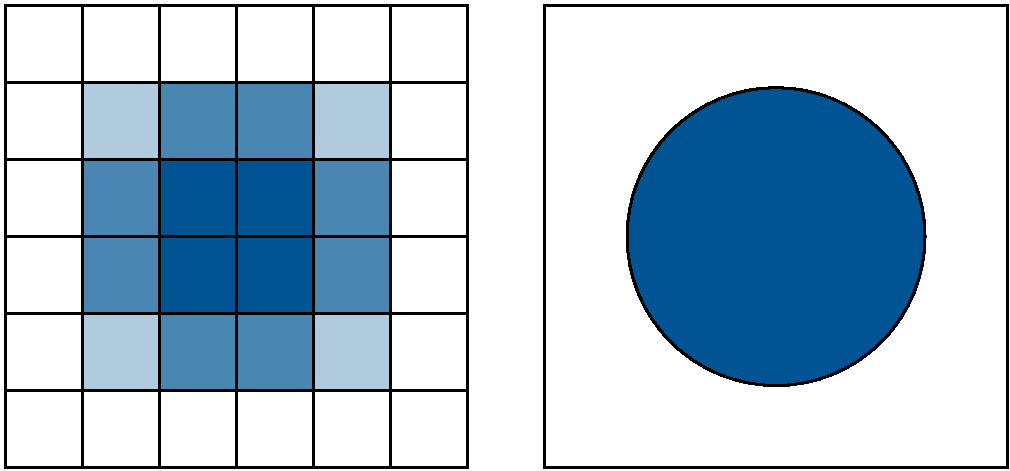
\includegraphics[width= 0.5\linewidth]{diagrams/vector-raster}
  \caption{The schematic difference between raster (left) and vector (right) graphics. }
  \label{fig:vector-raster}
\end{figure}

To save your output, you can use the typical R way with disk-based
graphics devices, which works for all packages, or a special function
from \texttt{ggplot} that saves the current plot: \texttt{ggsave()}.
\texttt{ggsave()} is optimised for interactive use and has the following
important arguments: \indexf{ggsave}

\begin{itemize}
\itemsep1pt\parskip0pt\parsep0pt
\item
  The \texttt{path} specifies the path where the image should be saved.
  The file extension will be used to automatically select the correct
  graphics device.
\item
  Three arguments control output size. If left blank, the size of the
  current on-screen graphics device will be used. \texttt{width} and
  \texttt{height} can be used to specify the absolute size, or
  \texttt{scale} to specify the size of the plot relative to the
  on-screen display. When creating the final versions of graphics it's a
  good idea to set \texttt{width} and \texttt{height} so you know
  exactly what size output you're going to get.
\item
  For raster graphics, the \texttt{dpi} argument controls the resolution
  of the plot. It defaults to 300, which is appropriate for most
  printers, but you may want to use 600 for particularly high-resolution
  output, or 72 for on-screen (e.g., web) display.
\end{itemize}

The following code shows these two methods. If you want to save multiple
plots to a single file, you will need to explicitly open a disk-based
graphics device (like \texttt{png()} or \texttt{pdf()}), print the plots
and then close it with \texttt{dev.off()}.

\begin{Shaded}
\begin{Highlighting}[]
\KeywordTok{qplot}\NormalTok{(mpg, wt, }\DataTypeTok{data =} \NormalTok{mtcars)}
\KeywordTok{ggsave}\NormalTok{(}\DataTypeTok{file =} \StringTok{"output.pdf"}\NormalTok{)}

\KeywordTok{pdf}\NormalTok{(}\DataTypeTok{file =} \StringTok{"output.pdf"}\NormalTok{, }\DataTypeTok{width =} \DecValTok{6}\NormalTok{, }\DataTypeTok{height =} \DecValTok{6}\NormalTok{)}
\CommentTok{# If inside a script, you will need to explicitly print() plots}
\KeywordTok{qplot}\NormalTok{(mpg, wt, }\DataTypeTok{data =} \NormalTok{mtcars)}
\KeywordTok{qplot}\NormalTok{(wt, mpg, }\DataTypeTok{data =} \NormalTok{mtcars)}
\KeywordTok{dev.off}\NormalTok{()}
\end{Highlighting}
\end{Shaded}

Table\textasciitilde{}\ref{tbl:graphic-recommendation} lists recommended
graphic formats for various tasks. R output generally works best as part
of a linux development tool chain: using png or pdf output in LaTeX
documents. With Microsoft Office it is easiest to use a high-resolution
(\texttt{dpi = 600}) png file. You can use vector output, but neither
Windows meta files nor postscript supports transparency, and while
postscript prints fine, it is only shown on screen if you add a preview
in another software package. Transparency is used to show confidence
intervals with the points showing through. If you copy and paste a graph
into Word, and see that the confidence interval bands have vanished,
that is the cause. The same advice holds for OpenOffice.
\index{Exporting!to Word} \index{Exporting!to Powerpoint}

If you are using LaTeX, I recommend including
\texttt{\textbackslash{}DeclareGraphicsExtensions\{.png,.pdf\}} in the
preamble. Then you don't need to specify the file extension in
\texttt{\textbackslash{}includegraphics\{\}} commands, but LaTeX will
pick png files in preference to pdf. \index{Exporting!to Latex} I choose
this order because you can produce all your files in pdf, and then go
back and re-render any big ones as png. Another useful command is
\texttt{\textbackslash{}graphicspath\{\}} which specifies a path in
which to look for graphics, allowing you to keep graphics in a separate
directory to the text.

\begin{table}
  \begin{center}
  \begin{tabular}{lll}
    \toprule
    Software & Recommended graphics device \\
    \midrule
    Illustrator & svg \\
    latex & ps \\
    MS Office & png (600 dpi) \\
    Open Office & png (600 dpi) \\
    pdflatex & pdf, png (600 dpi) \\
    web & png (72 dpi) \\
    \bottomrule 
  \end{tabular}
  \end{center}
  \caption{Recommended graphic output for different purposes.}
  \label{tbl:graphic-recommendation}
\end{table}

\hyperdef{}{sec:grid-layout}{\section{Multiple plots on the same
page}\label{sec:grid-layout}}

If you want to arrange multiple plots on a single page, you'll need to
learn a little bit of grid, the underlying graphics system used by
\texttt{ggplot}. The key concept you'll need to learn about is a
viewport: a rectangular subregion of the display. The default viewport
takes up the entire plotting region, and by customising the viewport you
can arrange a set of plots in just about any way you can imagine.
\index{Layout} \index{Publication!multiple plots on the same page}

To begin, let's create three plots that we can experiment with. When
arranging multiple plots on a page, it will usually be easiest to create
them, assign them to variables and then plot them. This makes it easier
to experiment with plot placement independent of content. The plots
created by the code below are shown in Figure \ref{fig:layout}.

\begin{Shaded}
\begin{Highlighting}[]
\NormalTok{(a <-}\StringTok{ }\KeywordTok{qplot}\NormalTok{(date, unemploy, }\DataTypeTok{data =} \NormalTok{economics, }\DataTypeTok{geom =} \StringTok{"line"}\NormalTok{))}
\NormalTok{(b <-}\StringTok{ }\KeywordTok{qplot}\NormalTok{(uempmed, unemploy, }\DataTypeTok{data =} \NormalTok{economics) +}\StringTok{ }
\StringTok{  }\KeywordTok{geom_smooth}\NormalTok{(}\DataTypeTok{se =} \NormalTok{F))}
\NormalTok{(c <-}\StringTok{ }\KeywordTok{qplot}\NormalTok{(uempmed, unemploy, }\DataTypeTok{data =} \NormalTok{economics, }\DataTypeTok{geom=}\StringTok{"path"}\NormalTok{))}
\end{Highlighting}
\end{Shaded}

\begin{figure}

{\centering \includegraphics[width=0.32\linewidth]{figures/polishinglayout-1} \includegraphics[width=0.32\linewidth]{figures/polishinglayout-2} \includegraphics[width=0.32\linewidth]{figures/polishinglayout-3} 

}

\caption{Three simple graphics we'll use to experiment with sophisticated plot layouts.\label{fig:layout}}
\end{figure}

\subsection{Subplots}

One common layout is to have a small subplot drawn on top of the main
plot. To achieve this effect, we first plot the main plot, and then draw
the subplot in a smaller viewport. Viewports are created with
(surprise!) the \texttt{viewport()} function, with parameters
\texttt{x}, \texttt{y}, \texttt{width} and \texttt{height} to control
the size and position of the viewport. By default, the measurements are
given in `npc' units, which range from 0 to 1. The location (0, 0) is
the bottom left, (1, 1) the top right and (0.5, 0.5) the centre of
viewport. If these relative units don't work for your needs, you can
also use absolute units, like \texttt{unit(2, "cm")} or
\texttt{unit(1, "inch")}. \index{Sub-figures} \index{Subplots}

\begin{Shaded}
\begin{Highlighting}[]
\CommentTok{# A viewport that takes up the entire plot device}
\NormalTok{vp1 <-}\StringTok{ }\KeywordTok{viewport}\NormalTok{(}\DataTypeTok{width =} \DecValTok{1}\NormalTok{, }\DataTypeTok{height =} \DecValTok{1}\NormalTok{, }\DataTypeTok{x =} \FloatTok{0.5}\NormalTok{, }\DataTypeTok{y =} \FloatTok{0.5}\NormalTok{)}
\NormalTok{vp1 <-}\StringTok{ }\KeywordTok{viewport}\NormalTok{()}

\CommentTok{# A viewport that takes up half the width and half the height, }
\CommentTok{# located in the middle of the plot.}
\NormalTok{vp2 <-}\StringTok{ }\KeywordTok{viewport}\NormalTok{(}\DataTypeTok{width =} \FloatTok{0.5}\NormalTok{, }\DataTypeTok{height =} \FloatTok{0.5}\NormalTok{, }\DataTypeTok{x =} \FloatTok{0.5}\NormalTok{, }\DataTypeTok{y =} \FloatTok{0.5}\NormalTok{)}
\NormalTok{vp2 <-}\StringTok{ }\KeywordTok{viewport}\NormalTok{(}\DataTypeTok{width =} \FloatTok{0.5}\NormalTok{, }\DataTypeTok{height =} \FloatTok{0.5}\NormalTok{)}

\CommentTok{# A viewport that is 2cm x 3cm located in the center}
\NormalTok{vp3 <-}\StringTok{ }\KeywordTok{viewport}\NormalTok{(}\DataTypeTok{width =} \KeywordTok{unit}\NormalTok{(}\DecValTok{2}\NormalTok{, }\StringTok{"cm"}\NormalTok{), }\DataTypeTok{height =} \KeywordTok{unit}\NormalTok{(}\DecValTok{3}\NormalTok{, }\StringTok{"cm"}\NormalTok{))}
\end{Highlighting}
\end{Shaded}

By default, the x and y parameters control the location of the centre of
the viewport. When positioning the plot in other locations, you may need
to use the \texttt{just} parameter to control which corner of the plot
you are positioning. The following code gives some examples.

\begin{Shaded}
\begin{Highlighting}[]
\CommentTok{# A viewport in the top right}
\NormalTok{vp4 <-}\StringTok{ }\KeywordTok{viewport}\NormalTok{(}\DataTypeTok{x =} \DecValTok{1}\NormalTok{, }\DataTypeTok{y =} \DecValTok{1}\NormalTok{, }\DataTypeTok{just =} \KeywordTok{c}\NormalTok{(}\StringTok{"right"}\NormalTok{, }\StringTok{"top"}\NormalTok{))}
\CommentTok{# Bottom left}
\NormalTok{vp5 <-}\StringTok{ }\KeywordTok{viewport}\NormalTok{(}\DataTypeTok{x =} \DecValTok{0}\NormalTok{, }\DataTypeTok{y =} \DecValTok{0}\NormalTok{, }\DataTypeTok{just =} \KeywordTok{c}\NormalTok{(}\StringTok{"right"}\NormalTok{, }\StringTok{"bottom"}\NormalTok{))}
\end{Highlighting}
\end{Shaded}

To draw the plot in our new viewport, we use the \texttt{vp} argument of
the \texttt{ggplot.print()} method. This method is normally called
automatically whenever you evaluate something on the command line, but
because we want to customise the viewport, we need to call it ourselves.
The result of this is shown in Figure \ref{fig:subplot-1}.

\begin{Shaded}
\begin{Highlighting}[]
\KeywordTok{pdf}\NormalTok{(}\StringTok{"figures/polishing-subplot-1.pdf"}\NormalTok{, }\DataTypeTok{width =} \DecValTok{4}\NormalTok{, }\DataTypeTok{height =} \DecValTok{4}\NormalTok{)}
\NormalTok{subvp <-}\StringTok{ }\KeywordTok{viewport}\NormalTok{(}\DataTypeTok{width =} \FloatTok{0.4}\NormalTok{, }\DataTypeTok{height =} \FloatTok{0.4}\NormalTok{, }\DataTypeTok{x =} \FloatTok{0.75}\NormalTok{, }\DataTypeTok{y =} \FloatTok{0.35}\NormalTok{)}
\NormalTok{b}
\KeywordTok{print}\NormalTok{(c, }\DataTypeTok{vp =} \NormalTok{subvp)}
\KeywordTok{dev.off}\NormalTok{()}
\end{Highlighting}
\end{Shaded}

This gives us what we want, but we need to make a few tweaks to the
appearance: the text should be smaller, we want to remove the axis
labels and shrink the plot margins. The result is shown in Figure
\ref{fig:subplot-2}.

\begin{Shaded}
\begin{Highlighting}[]
\NormalTok{csmall <-}\StringTok{ }\NormalTok{c +}\StringTok{ }
\StringTok{  }\KeywordTok{theme_gray}\NormalTok{(}\DecValTok{9}\NormalTok{) +}\StringTok{ }
\StringTok{  }\KeywordTok{labs}\NormalTok{(}\DataTypeTok{x =} \OtherTok{NULL}\NormalTok{, }\DataTypeTok{y =} \OtherTok{NULL}\NormalTok{) +}\StringTok{ }
\StringTok{  }\KeywordTok{theme}\NormalTok{(}\DataTypeTok{plot.margin =} \KeywordTok{unit}\NormalTok{(}\KeywordTok{c}\NormalTok{(}\DecValTok{1}\NormalTok{/}\DecValTok{4}\NormalTok{, }\DecValTok{0}\NormalTok{, }\DecValTok{0}\NormalTok{, }\DecValTok{0}\NormalTok{), }\StringTok{"lines"}\NormalTok{))}

\KeywordTok{pdf}\NormalTok{(}\StringTok{"figures/polishing-subplot-2.pdf"}\NormalTok{, }\DataTypeTok{width =} \DecValTok{4}\NormalTok{, }\DataTypeTok{height =} \DecValTok{4}\NormalTok{)}
\NormalTok{b}
\KeywordTok{print}\NormalTok{(csmall, }\DataTypeTok{vp =} \NormalTok{subvp)}
\KeywordTok{dev.off}\NormalTok{()}
\end{Highlighting}
\end{Shaded}

\begin{figure}[htbp]
  \centering
  \subfigure[Figure with subplot.]{
    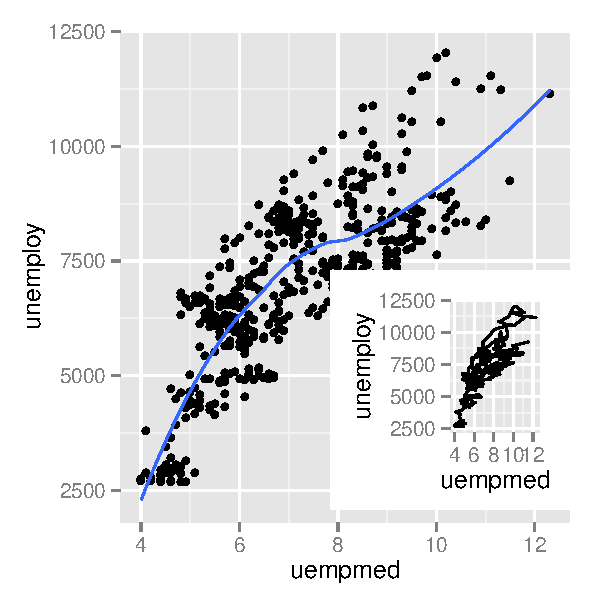
\includegraphics[width=0.5\textwidth]{figures/polishing-subplot-1}
    \label{fig:subplot-1}
  }%
  \subfigure[Subplot tweaked for better display.]{
    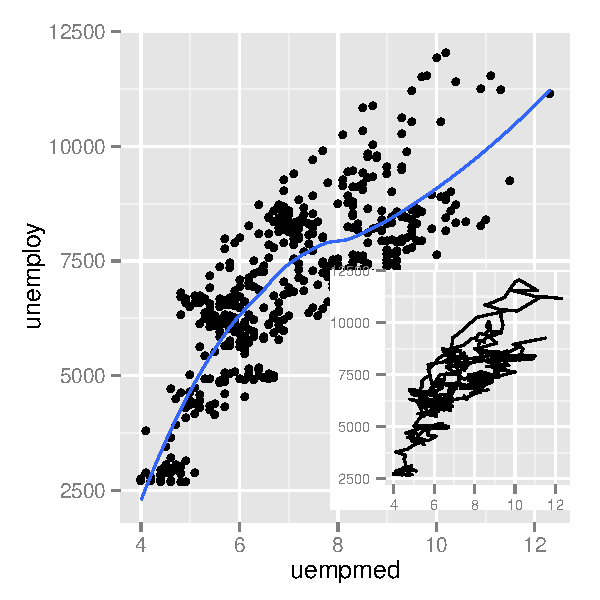
\includegraphics[width=0.5\textwidth]{figures/polishing-subplot-2}
    \label{fig:subplot-2}
  }
  \caption{Two examples of a figure with subplot. It will usually be necessary to tweak the theme settings of the subplot for optimum display.}
  \label{fig:subplot}
\end{figure}

Note we need to use \texttt{pdf()} (or \texttt{png()} etc.) to save the
plots to disk because \texttt{ggsave()} only saves a single plot.

\subsection{Rectangular grids}

A more complicated scenario is when you want to arrange a number of
plots in a rectangular grid. Of course you could create a series of
viewports and use what you've learned above, but doing all the
calculations by hand is cumbersome. A better approach is to use
\texttt{grid.layout()}, which sets up a regular grid of viewports with
arbitrary heights and widths. You still need to create each viewport,
but instead of explicitly specifying the position and size, you can
specify the row and column of the layout.

The following example shows how this work. We first create the layout,
here a 2 by 2 grid, then assign it to a viewport and push that viewport
on to the plotting device. Now we are ready to draw each plot into its
own position on the grid. We create a small function to save some
typing, and then draw each plot in the desired place on the grid. You
can supply a vector of rows or columns to span a plot over multiple
cells. The results are shown in Figure \ref{fig:layout-2}.

\begin{Shaded}
\begin{Highlighting}[]
\KeywordTok{grid.newpage}\NormalTok{()}
\KeywordTok{pushViewport}\NormalTok{(}\KeywordTok{viewport}\NormalTok{(}\DataTypeTok{layout =} \KeywordTok{grid.layout}\NormalTok{(}\DecValTok{2}\NormalTok{, }\DecValTok{2}\NormalTok{)))}

\NormalTok{vplayout <-}\StringTok{ }\NormalTok{function(x, y) }
  \KeywordTok{viewport}\NormalTok{(}\DataTypeTok{layout.pos.row =} \NormalTok{x, }\DataTypeTok{layout.pos.col =} \NormalTok{y)}
\KeywordTok{print}\NormalTok{(a, }\DataTypeTok{vp =} \KeywordTok{vplayout}\NormalTok{(}\DecValTok{1}\NormalTok{, }\DecValTok{1}\NormalTok{:}\DecValTok{2}\NormalTok{))}
\KeywordTok{print}\NormalTok{(b, }\DataTypeTok{vp =} \KeywordTok{vplayout}\NormalTok{(}\DecValTok{2}\NormalTok{, }\DecValTok{1}\NormalTok{))}
\KeywordTok{print}\NormalTok{(c, }\DataTypeTok{vp =} \KeywordTok{vplayout}\NormalTok{(}\DecValTok{2}\NormalTok{, }\DecValTok{2}\NormalTok{))}
\end{Highlighting}
\end{Shaded}

\begin{figure}

{\centering \includegraphics[width=\linewidth]{figures/polishinglayout-2-1} 

}

\caption{Three plots laid out in a grid using \texttt{grid.layout()}.\label{fig:layout-2}}
\end{figure}

By default \texttt{grid.layout()} makes each cell the same size, but you
can use the \texttt{widths} and \texttt{heights} arguments to make them
different sizes. See the documentation for \texttt{grid.layout()} for
more examples.

Brewer, Cynthia A. 1994. ``Color Use Guidelines for Mapping and
Visualization.'' In \emph{Visualization in Modern Cartography}, edited
by A.M. MacEachren and D.R.F. Taylor, 123--47. Elsevier Science.

Carr, Dan. 1994. ``Using Gray in Plots.'' \emph{ASA Statistical
Computing and Graphics Newsletter} 2 (5): 11--14.
\url{http://www.galaxy.gmu.edu/~dcarr/lib/v5n2.pdf}.

---------. 2002. ``Graphical Displays.'' In \emph{Encyclopedia of
Environmetrics}, edited by Abdel H. El-Shaarawi and Walter W. Piegorsch,
2:933--60. John Wiley \& Sons.
\url{http://www.galaxy.gmu.edu/~dcarr/lib/EnvironmentalGraphics.pdf}.

Carr, Dan, and Ru Sun. 1999. ``Using Layering and Perceptual Grouping in
Statistical Graphics.'' \emph{ASA Statistical Computing and Graphics
Newsletter} 10 (1): 25--31.

Cleveland, William. 1993. ``A Model for Studying Display Methods of
Statistical Graphics.'' \emph{Journal of Computational and Graphical
Statistics} 2: 323--64. \url{http://stat.bell-labs.com/doc/93.4.ps}.

Tufte, Edward R. 1990. \emph{Envisioning Information}. Graphics Press.

---------. 1997. \emph{Visual Explanations}. Graphics Press.

---------. 2001. \emph{The Visual Display of Quantitative Information}.
second. Graphics Press.

---------. 2006. \emph{Beautiful Evidence}. Graphics Press.
